\documentclass[final]{beamer}

\usepackage[T1]{fontenc}
\usepackage[czech]{babel}
\usepackage{lmodern}
\usepackage[size=a3paper,scale=1.2]{beamerposter}
\usetheme{gemini}
\usecolortheme{mit}
\usepackage{graphicx}
\usepackage{booktabs}
\usepackage{tikz}
\usepackage{pgfplots}
\usepackage{subfigure}
\pgfplotsset{compat=1.14}

% ====================
% Lengths
% ====================

% If you have N columns, choose \sepwidth and \colwidth such that
% (N+1)*\sepwidth + N*\colwidth = \paperwidth
\newlength{\sepwidth}
\newlength{\colwidth}
\setlength{\sepwidth}{0.025\paperwidth}
\setlength{\colwidth}{0.3\paperwidth}

\newcommand{\separatorcolumn}{\begin{column}{\sepwidth}\end{column}}

% ====================
% Title
% ====================

\title{Maturitní práce -- Bezpilotní letadlo}

\author{Havránek Kryštof (Programování, 4.E)}

\institute[shortinst]{Gymnázium, Praha 6, Arabská 14}

% ====================
% Footer (optional)
% ====================

\footercontent{
  \href{https://github.com/havrak/UAV-project}{https://github.com/havrak/UAV-project} \hfill
  Březen 2022 \hfill
  \href{mailto:krystof@havrak.xyz}{krystof@havrak.xyz}}
% (can be left out to remove footer)

% ====================
% Logo (optional)
% ====================

% use this to include logos on the left and/or right side of the header:
\logoleft{
\includegraphics[height=7cm]{logo.png}}
% \logoleft{\includegraphics[height=7cm]{logo2.pdf}}

% ====================
% Body
% ====================

\begin{document}

\begin{frame}[t]
  \begin{columns}[t]
    \separatorcolumn

    \begin{column}{\colwidth}

      \begin{block}{Abstrakt}

        Cílem práce je vytvoření bezpilotního letadla a doprovodného systému umožnující pilotovi letadlo dálkově ovládat.
        Pilot by měl mít možnost sledovat živý přenos z kamery a získávat doprovodnou telemetrii.
        Celý program by měl být rychlý, aby ovládání bylo s co nejmenší odezvou, a napsaný stylem umožnující další vývoj.

      \end{block}

      \begin{block}{Použité technologie}

        \begin{figure}
          \subfigure{
\includegraphics[width=4.5cm]{./index1.png}}
          \hfill
          \subfigure{
\includegraphics[width=6cm]{./index2.png}}
          \hfill
          \subfigure{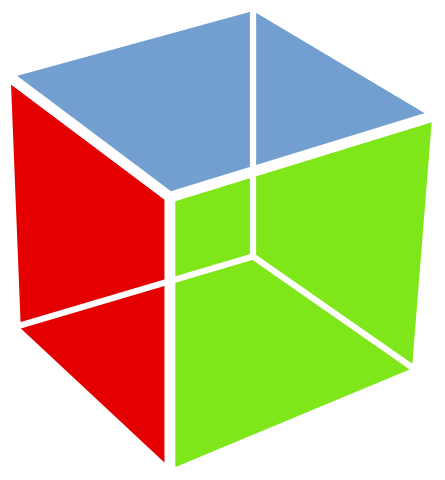
\includegraphics[width=4.5cm]{./index3.png}}
          \hfill
          \subfigure{
\includegraphics[width=4.5cm]{./index4.png}}
          \hfill
          \subfigure{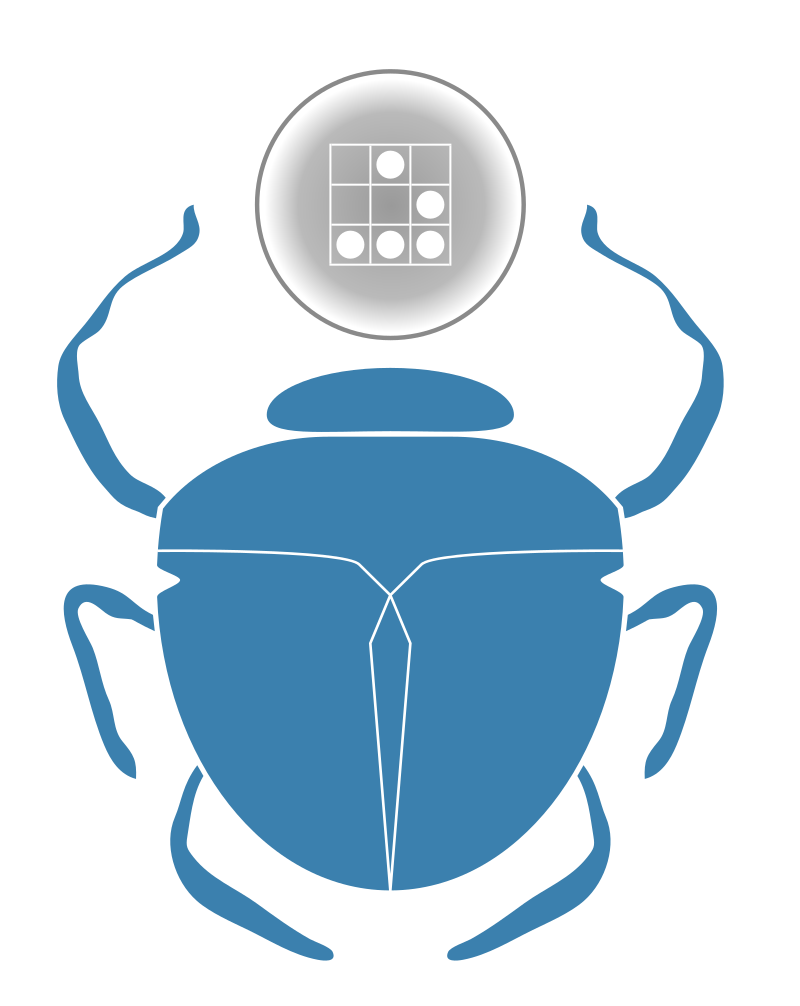
\includegraphics[width=4.5cm]{./index6.png}}
          \hfill
          \subfigure{
\includegraphics[width=4.5cm]{./index5.jpg}}
          \hfill

        \end{figure}

			Celý projekt je psán v jazyce C++ a vyvíjen primárně pro zařízení s operačním systémem Linux.
			V případě ovládací softwaru je port na další OS možný, jelikož používaný grafický toolikt je multiplatformní.



      \end{block}

      \begin{block}{Komunikační protokol}

				Obě části projektu mezi sebou komunikují prostřednictvím protokolu postaveném na rodině TCP.
				Letadlo na sebe přejímá roli serveru, umožňuje tak několik clientů -- telemetrii z dronu lze tak monitorovat z několika počítačů.
				Případně si lze \uv{předávat} kontrolu nad dronem mezi počítači.

				Protokol se stará o tři důležité části řízení letadla.
				Je schopen na dálku drona konfigurovat -- například spustit kameru.
				Dále předává informace letadlu z herního, kterým se letadlo ovládá.
				V neposlední řadě umožňuje letadlu posílat zpět telemetrii, případě chybové hlášky.
				Telemetrie se pak zobrazuje pilotu v ovládacím softwaru, chybové hlášky se manifestují prostřednictvím dialogových oken.
      \end{block}

      \begin{block}{Fotografie letadla}


				\begin{figure}[h]
					\centering
					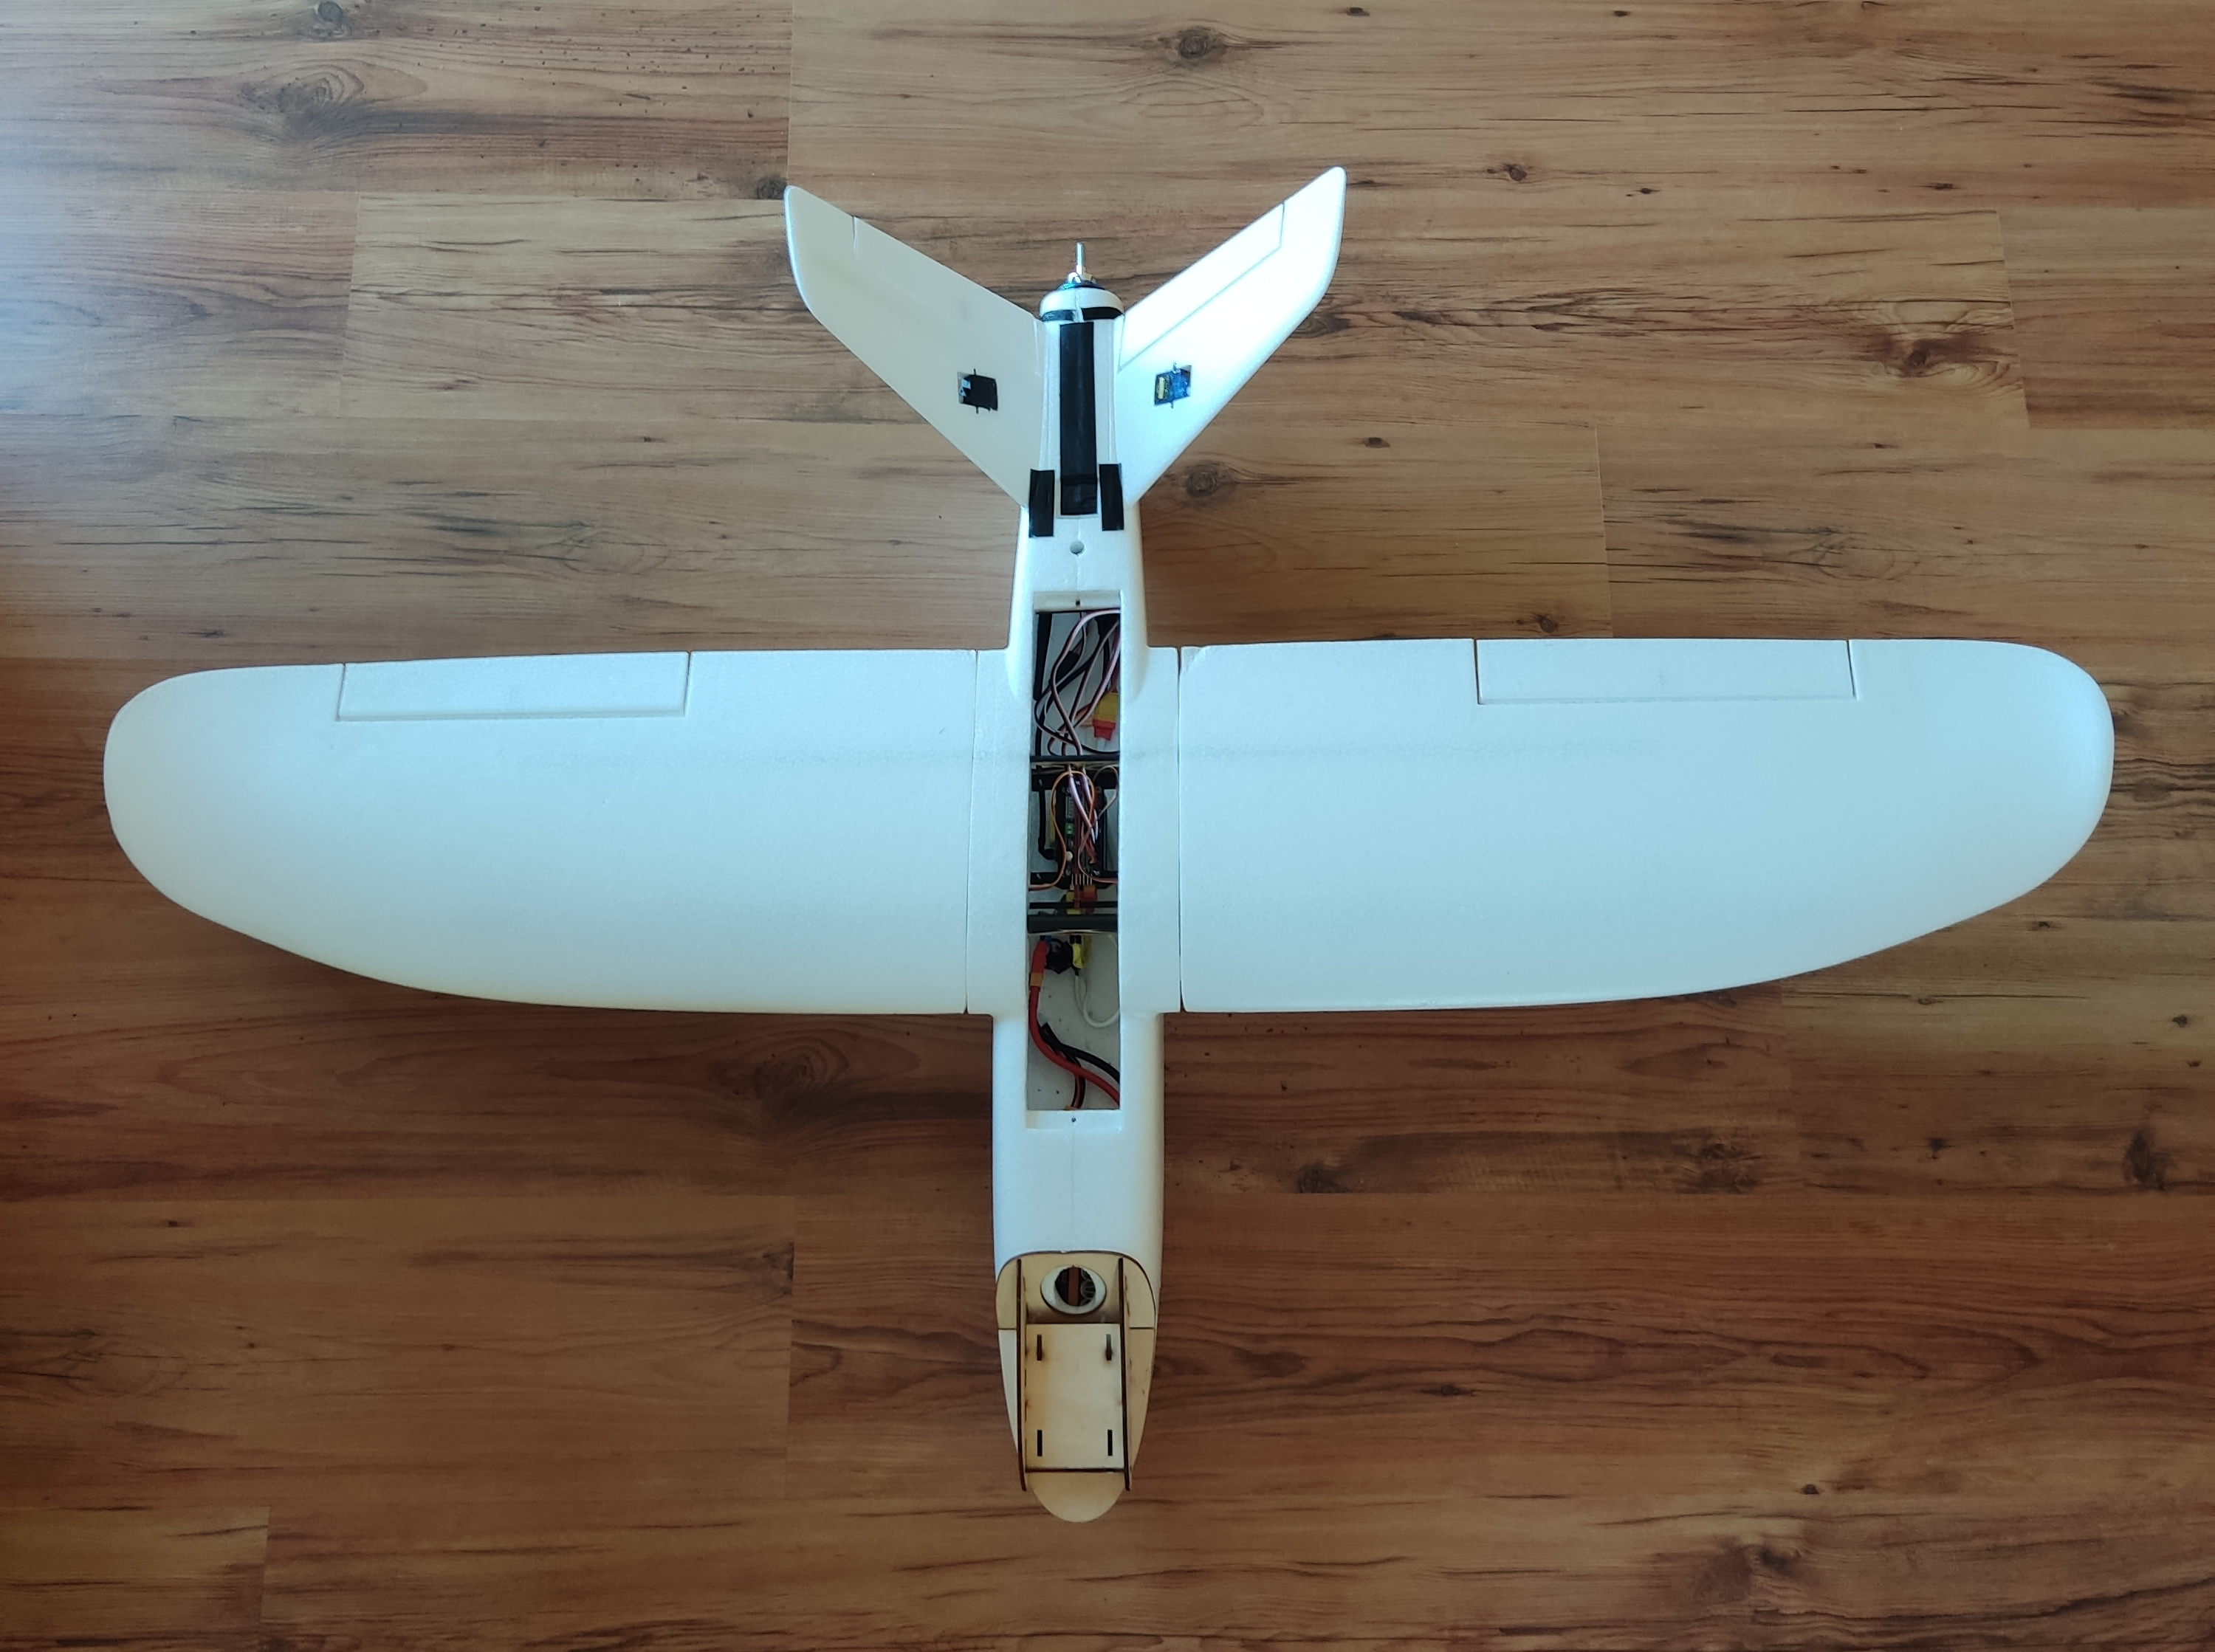
\includegraphics[height=19cm]{../img/whole_plane.jpg}
				\end{figure}

      \end{block}

    \end{column}

    \separatorcolumn

    \begin{column}{\colwidth}

      \begin{block}{Hardware a software letadla}

				Dron je postaven na jednodeskovém počítači Raspberry Pi.
				Systém je primárně určen pro moduly ze série Raspberry Pi Zero.
				Primárně se však tak je činěno z důvodu prostorových omezení řad koster letadel.
				Teoreticky může projekt fungovat na libovolném počítači Raspberry Pi.

				Jelikož používá specifické funkce pro interakci s hardwarem není možné projekt rozeběhnout na dalších malých počítačích.
				Stejně tak je projekt závislý na knihovnách a driverech, které jsou standardní součástí operačního systému raspbian.

				Projekt využívá hned několik periférií, těma jsou:

        \begin{enumerate}
          \item WT901B -- devíti-osý polohový senzor -- počítá yaw, roll a pitch
          \item PCA9865 -- modul pro ovládání servo motorů
          \item INA226 -- voltmetr/ampérmetr pro získání dat z baterie
					\item ublox NEO 7M GPS -- GPS modul
					\item Beatles 40A ESC -- Electronic Speed Control -- umožňuje ovládat hlavní motor
        \end{enumerate}

      \end{block}

      \begin{block}{Schéma zapojení}

				Schéma zapojení je relativně přímočaré.
				Většina komponent s Raspberry PI komunikuje prostřednictvím I2C spojený a je napojena na piny 3 a 5.
				Vzhledem k počtu komponent jsou napojené na 3.3V drain přes 4.7 $\Omega$ rezistory.
				Výjimku představuje GPS, která využívá sériovou linku.

				Raspberry Pi a další sensory nejsou napájené prostřednictvím ESC, ale z přímo baterie prostřednictvím DC/DC step down covertru.

				\begin{figure}[h]
					\centering
					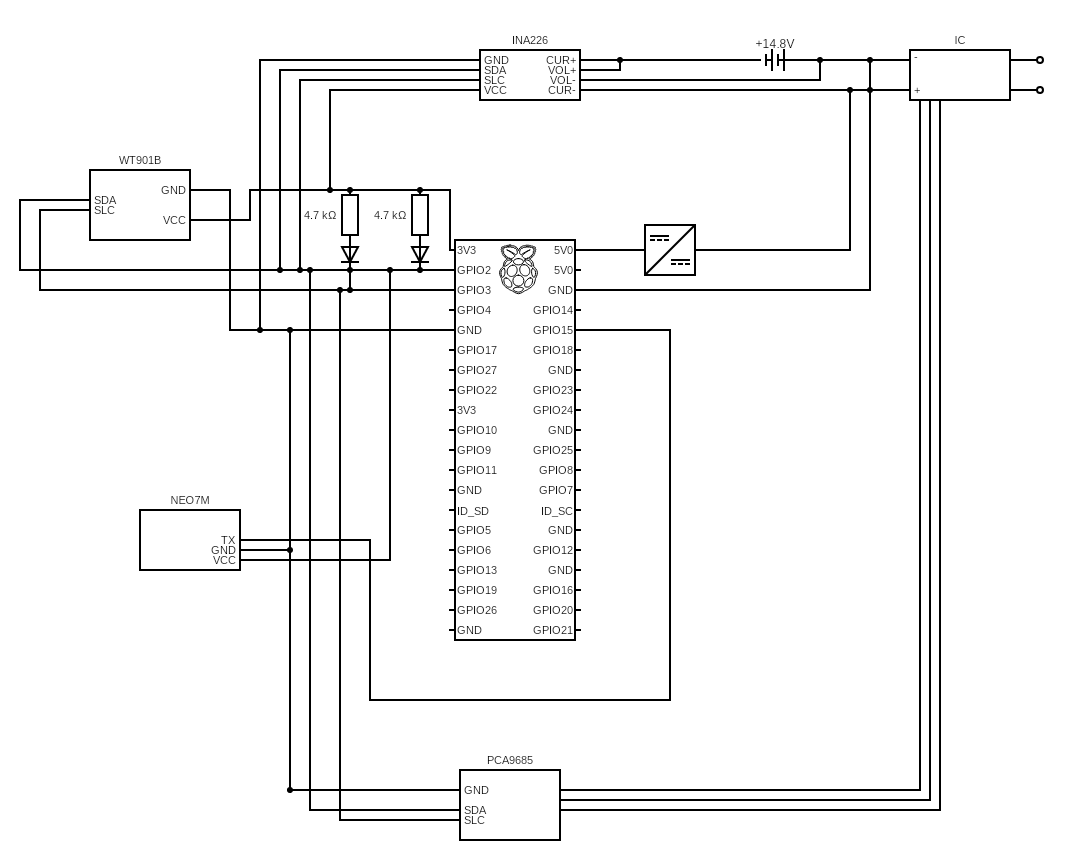
\includegraphics[height=27cm]{../img/schema.png}
				\end{figure}


      \end{block}

    \end{column}

    \separatorcolumn

    \begin{column}{\colwidth}

			\begin{block}{Zapojení}

				Většina komponent je umístěna na pájivém poli, které se přímo nasazuje na samotné Raspberry Pi.
				Voltmetr se nachází v ocasní části letadla, je tak separátně od většiny komponent a připojuje se k nim prostřednictvím USB konektoru.

				K Raspberry Pi je také připojen Wi-Fi Adaptér, který poskytuje silnější signál než integrovaný Wi-Fi čip.
				To jest potřeba, jelikož dron funguje jako router.

				\begin{figure}[h]
					\centering
					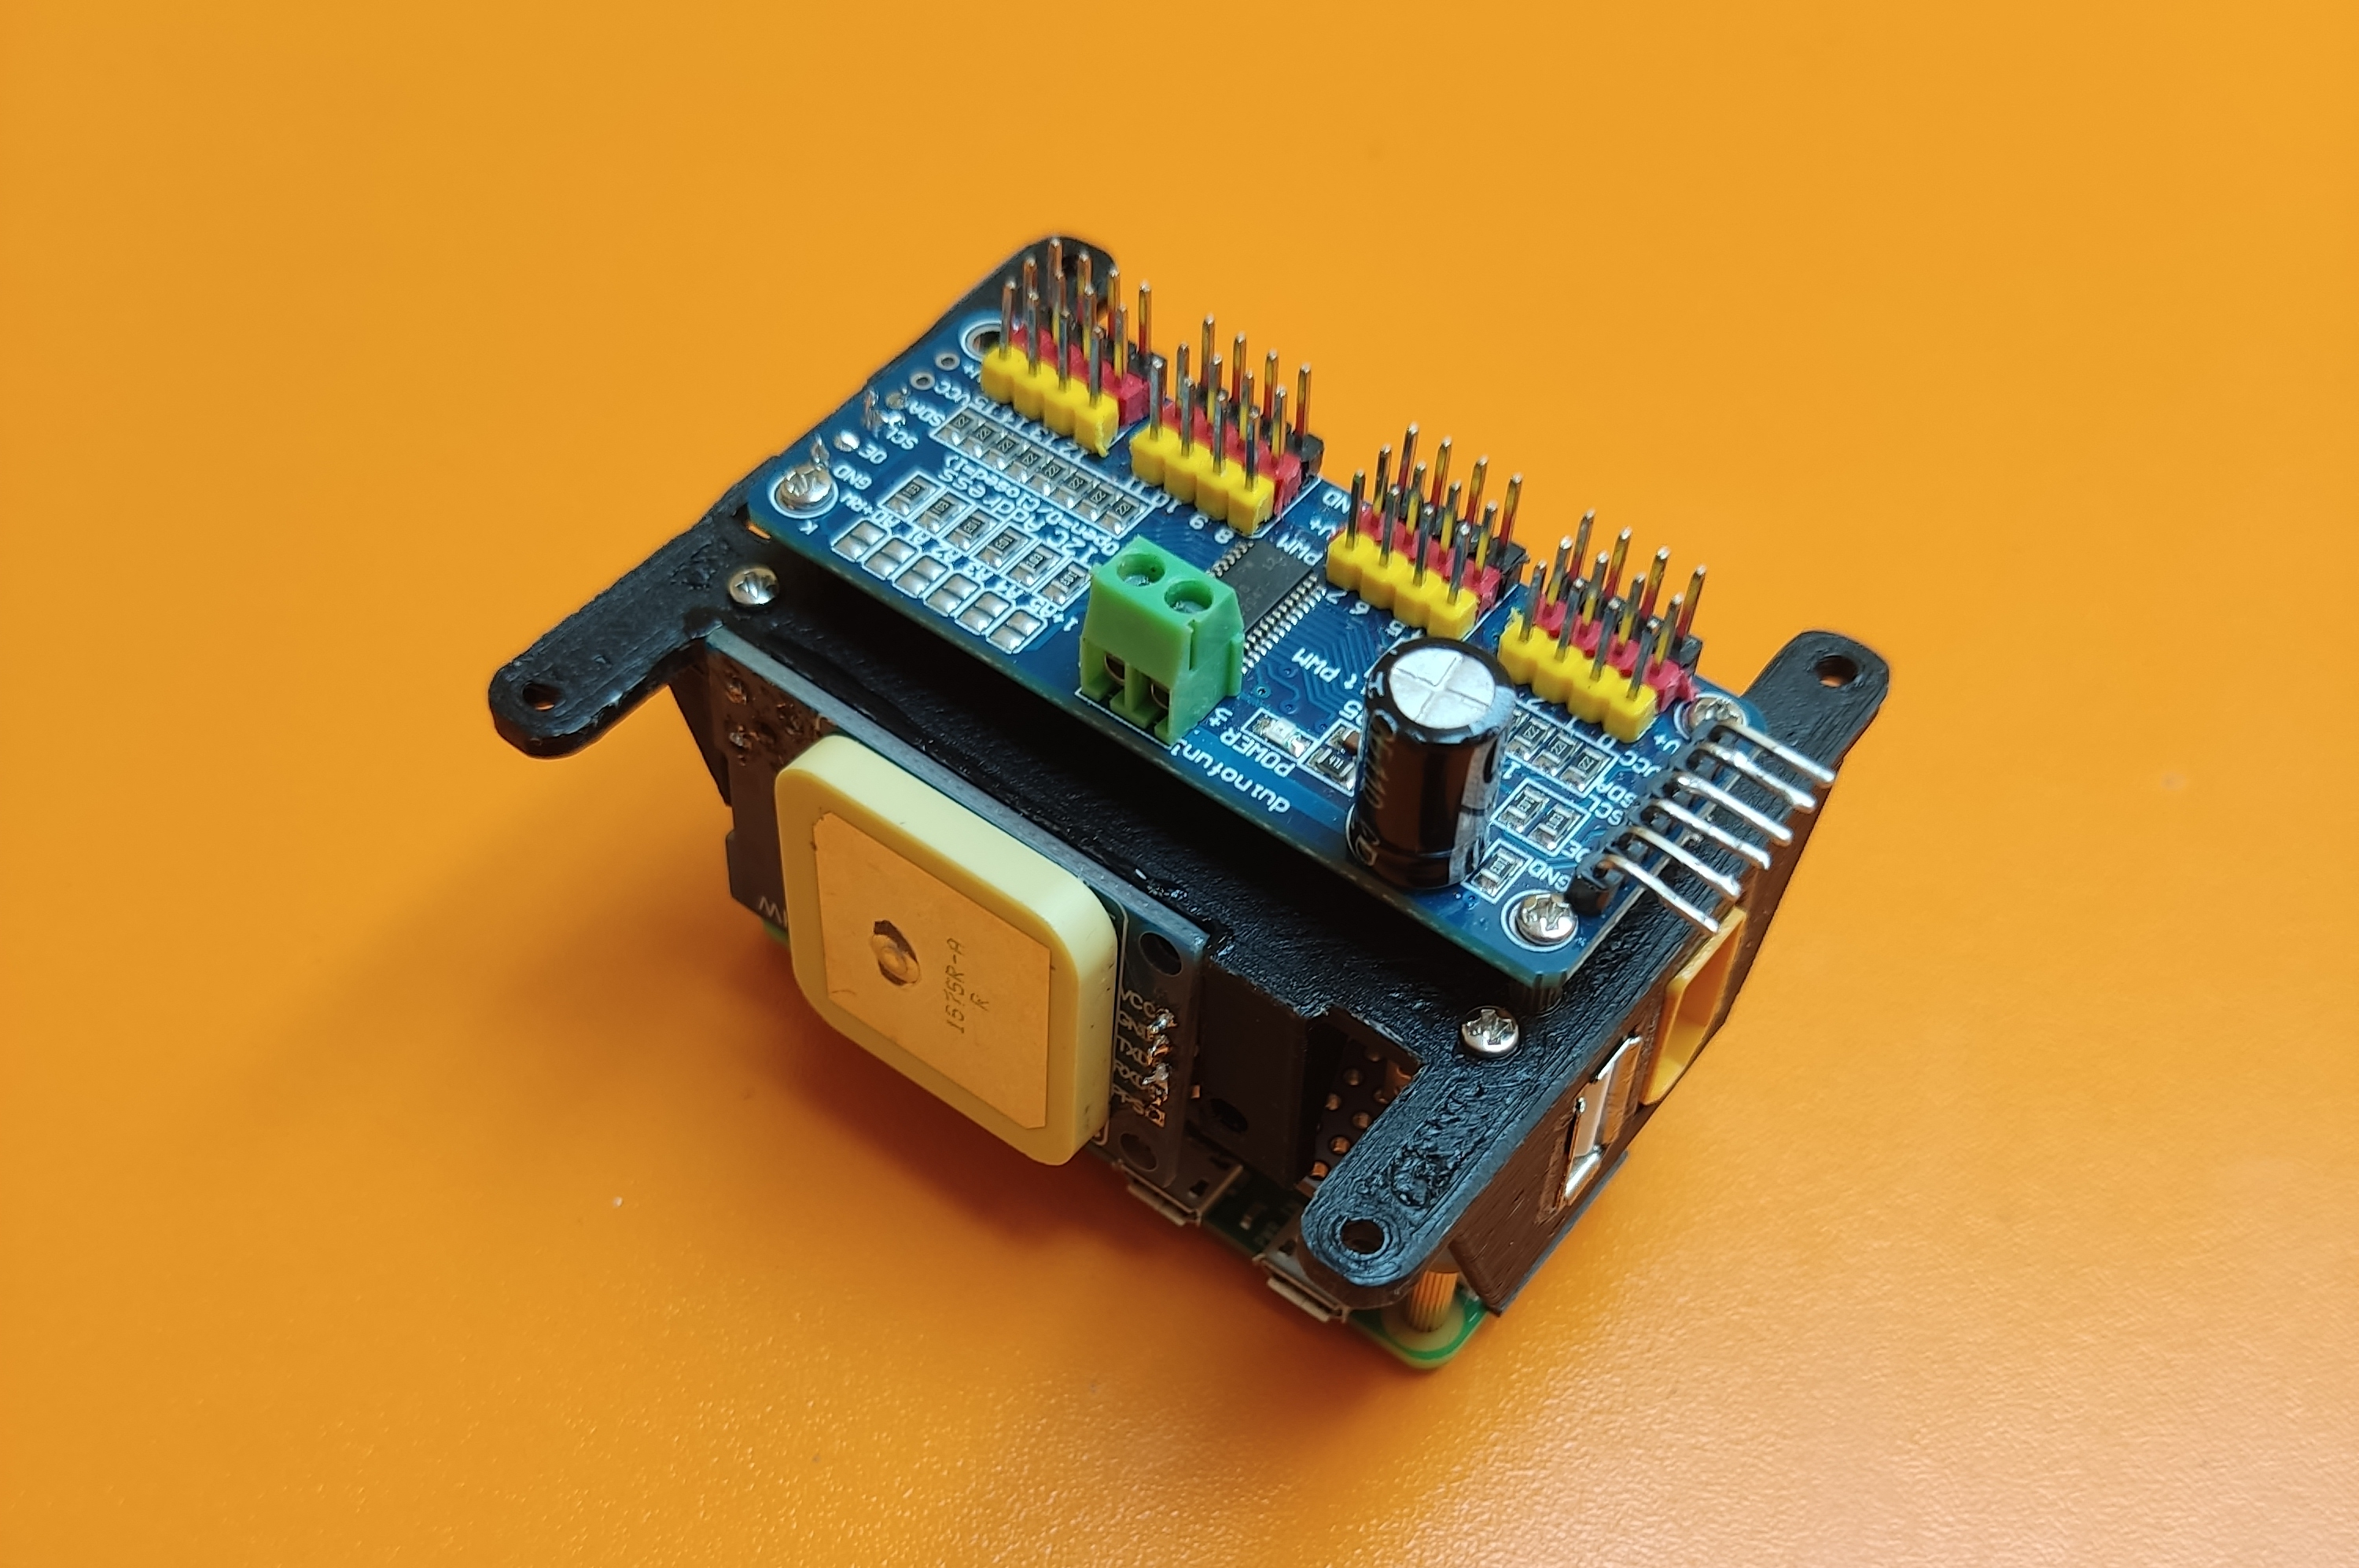
\includegraphics[height=19cm]{../img/detail.jpg}
				\end{figure}

			\end{block}



			\begin{block}{Ovládání}

				Letadlo se ovládá pomocí ovladače od herní konzole Xbox One.
				Poloha prvků ovladače je posílána přímo na letadlo, kde se teprve interpretuje.
				Nejprve se přepočítají polohy joysticků na čtverec a pak se vyvodí polohy 4 ovládacích ploch (2 $\times$ aileron, 2 $\times$ ruddervator)

				\underline{Autopilot:}

				Letadlo je schopno držet svojí letovou hladinu bez zásahu pilota.
				K tomu slouží jednoduchý autopilot postavený na dvou PID (proporčně-integračně-derivačních) kontrolérech.
				Jeden se snaží minimalizovat yaw letadla, druhý pak jeho pitch.

			\end{block}

      \begin{block}{Software pro řízení letadla}

			\begin{columns}[T]
				\begin{column}{.4\textwidth}
					Dron se řídí prostřednictvím jednoduché aplikace pro počítač.
					Grafické prostředí je psáno s pomocí knihovny Gtk3, dobře tak ladí s většinou dalších oken na Linuxu.
					Aplikace aktuálně pouze zobrazuje telemetrii z dronu a záznam z jeho kamery.
					Další funkce nebyly zatím implementovány.

				\end{column}
				\begin{column}{.6\textwidth}
			\begin{figure}[h]
				\centering
				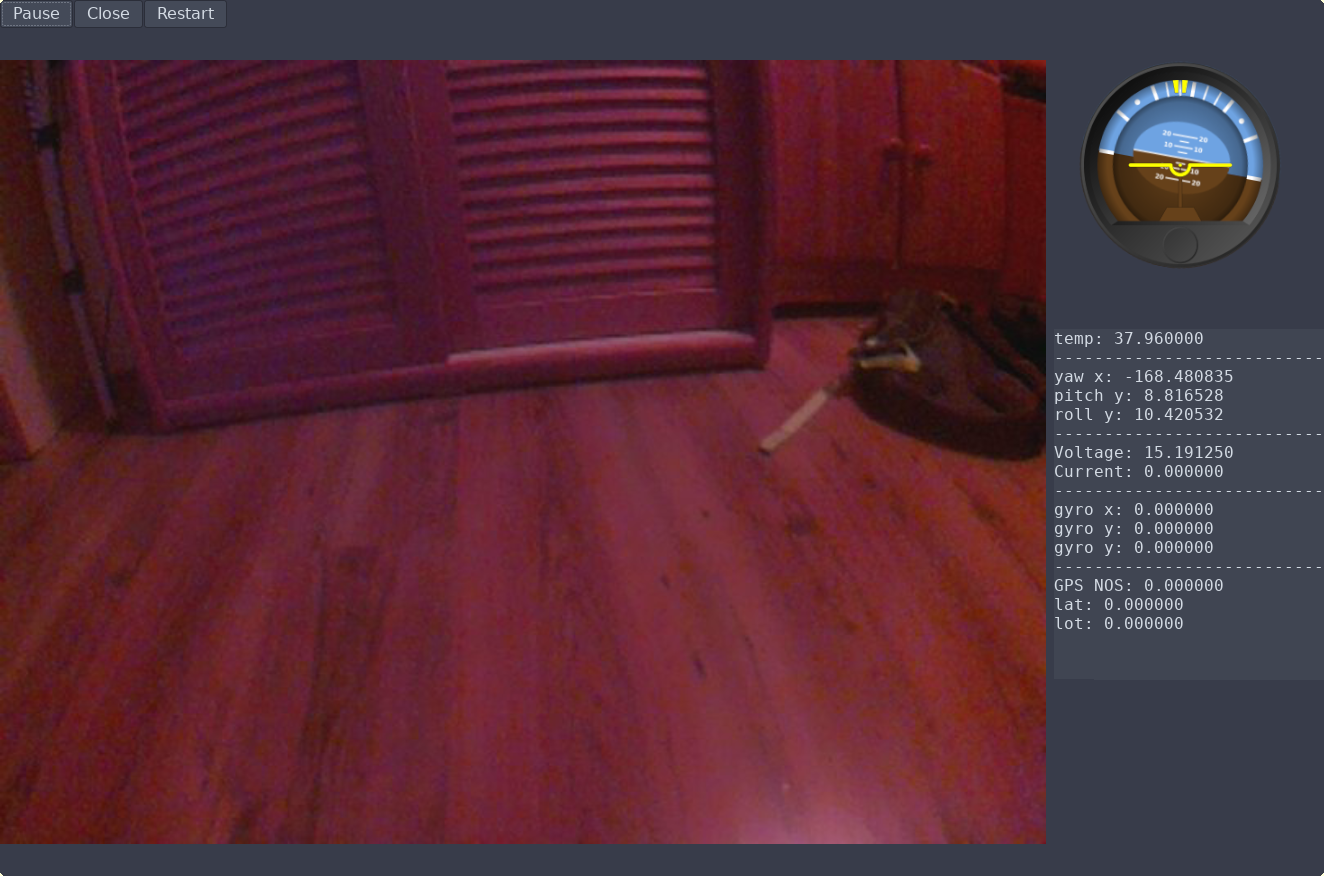
\includegraphics[height=12cm]{../img/interface.png}
			\end{figure}

				\end{column}
			\end{columns}



      \end{block}

    \end{column}

    \separatorcolumn
  \end{columns}
\end{frame}

\end{document}
